\scanpage{20}
\mspage{\textcircled{3}}

\begin{center}
\uline{ACADEMIE D'AIX-MARSEILLE}\\
INSPECTION ACADEMIQUE\\
\uline{DE VAUCLUSE}
\end{center}

\diagram{\begin{tikzcd}[ampersand replacement=\&,column sep=large,row sep=small]
{}\&\unsure{\mathfrak S_2|\mathcal G_2}\&\unsure{\mathfrak S_3|\mathcal G_3}\\
X_1\arrow[r,bend right=55,"\delta_0"']\&X_2\arrow[l,shift right=1.2,"p_0"']\arrow[l,shift left=1.2,"p_1"]\arrow[r,bend right=45,"\delta_1"']\arrow[r,bend right=60,"\delta_2"']\arrow[r,bend right=75,"\delta_3"']\&X_3\arrow[l,shift right=3,"p_{12}"']\arrow[l,"p_{23}"']\arrow[l,shift left=3,"p_{31}"]
\end{tikzcd}}
\margin{$\rho,\sigma_1,\sigma_2,\sigma_3$}
\deleted{$p=q$}

\figure{\begin{tikzpicture}
\node at (0,0) {\diagram{\begin{tikzcd}[ampersand replacement=\&,column sep=large,row sep=large]
X_2\arrow[r,two heads,"{(p_0,p_1)\ \text{épi}}"]\&X_1\times X_1\\
{}\&X_1\arrow[u,hook]\arrow[ul,"\delta_0"']
\end{tikzcd}}};
\node at (-2.6,.5) {$\unsure{\mathfrak S_2|\mathcal G_2}$};
\node at (.15,1.5) {$\begin{gathered}p_0\sigma\\\Vert\end{gathered}$};
\draw (-1.8,1.65)--(2.1,1.8)..controls(2.5,1.8)and(2.5,1.8)..(2.5,1.3);\draw(2.5,1.1)--(2.7,-.15)..controls(2.7,-.4)and(2.3,-.4)..(-1.8,-.5);\draw(-1.8,-.5)--(-1.8,.9);
\node at (-1.6,-2) {iso ???};\draw (-1.6,-2) ellipse (1 and .5);
\draw[->] (-.3,.3)..controls(-.8,-.8)and(-2.8,-1.4)..(-2.3,-1.85);
\end{tikzpicture}}

\diagram{\begin{tikzcd}[ampersand replacement=\&,column sep=large]
X_3\arrow[r,two heads,"{(p_{12},\unsure{q_3})\ \text{épi}}"]\&X_2\times X_1\arrow[r,two heads,"{(p_0,p_1)\times\mathrm{id}_{X_1}}"]\&X_1\times X_1\times X_1
\end{tikzcd}}
\diagram{\begin{tikzcd}[ampersand replacement=\&,column sep=large]
X_3\arrow[r,two heads,"\text{épi}","{(p_{12},p_{23})}"']\&\overset{(p_1)}{X_2}\times_{X_1}\overset{(p_0)}{X_2}\arrow[r,two heads,"\text{épi}"]\&X_2\times_{X_1}(X_1\times X_1)
\end{tikzcd}}

\diagram{\begin{tikzcd}[ampersand replacement=\&]
\mathbb E_1\arrow[r]\arrow[d]\&\mathbb E_2\arrow[d]\\
\mathbb E_2\arrow[r]\&\mathbb E_3
\end{tikzcd}}
\figure{
\begin{tikzpicture}
\fill (0,0) circle (.04);\fill(.5,0) circle(.04);\fill(1,0)circle(.04);
\draw(0,-.18)..controls(.05,-.35)and(.2,-.35)..(.25,-.23)..controls(.35,-.35)and(.5,-.35)..(.5,-.18);
\draw(.5,.16)..controls(.55,.35)and(.7,.35)..(.75,.23)..controls(.85,.35)and(1,.35)..(1,.16);
\end{tikzpicture}}
\diagram{\begin{tikzcd}[ampersand replacement=\&]
\mathbb E_3\arrow[r,"K_2"]\arrow[d,"K'_2"']\&\mathbb E_2\arrow[d,"K_1"]\\
\mathbb E_2\arrow[r,"K_1"]\&\mathbb E_1
\end{tikzcd}}

\figure{\begin{tikzpicture}
\node at (0,0) {\diagram{\begin{tikzcd}[ampersand replacement=\&,column sep=large,row sep=large]
X_3\arrow[r,two heads,"\unsure{p_1|\delta_1}"]\&X_2\\
X_{\unsure{2}}\arrow[u,hook,"\delta_3"]\arrow[ur,phantom,"\text{cart}"]\&X_1\arrow[l,hook,"\delta_0"]\arrow[u,hook,"\delta_0"']
\end{tikzcd}}};\draw (0,0) ellipse (2.9 and 1.9);
\end{tikzpicture}}

\diagram{\begin{tikzcd}[ampersand replacement=\&]
\mathbb E_2\arrow[r,dash,"\delta_{\unsure{3|2}}"]\arrow[d,"K_{\unsure{1}}"']\&\mathbb E_3\arrow[d,"K'_2"]\\
\mathbb E_1\arrow[r,"\delta_1"]\&\mathbb E_2
\end{tikzcd}}

\deleted{\figure{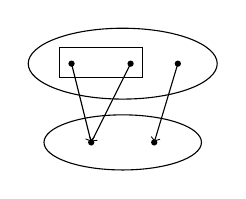
\begin{tikzpicture}
\draw(0,0)ellipse(1.2 and .45);\draw(-.8,-.18)rectangle(.25,.20);\fill(-.65,0)circle(.04);\fill(.1,0)circle(.04);\fill(.7,0)circle(.04);
\draw(0,-1)ellipse(1 and .35);\fill(-.4,-1)circle(.04);\fill(.4,-1)circle(.04);
\draw[->](-.65,0)--(-.4,-1);\draw[->](.1,0)--(-.4,-1);\draw[->](.7,0)--(.4,-1);
\end{tikzpicture}}}
\figure{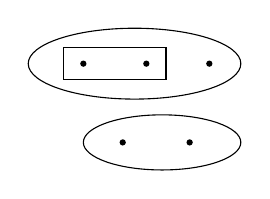
\begin{tikzpicture}
\draw(0,0)ellipse(1.35 and .45);\draw(-.9,-.2)rectangle(.4,.2);\fill(-.65,0)circle(.04);\fill(.15,0)circle(.04);\fill(.95,0)circle(.04);
\draw(.35,-1)ellipse(1 and .35);\fill(-.15,-1)circle(.04);\fill(.7,-1)circle(.04);
\end{tikzpicture}}
\deleted{\figure{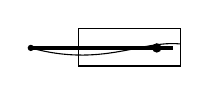
\begin{tikzpicture}
\draw[very thick](-.7,0)--(1.1,0);\fill(-.7,0)circle(.04);\fill(.9,0)circle(.06);\draw(-.1,-.23)rectangle(1.2,.25);\draw(-.7,0)..controls(.2,-.25)and(.7,.1)..(1.2,.05);
\end{tikzpicture}}}

\figure{\begin{tikzpicture}
\node at (0,0) {\diagram{\begin{tikzcd}[ampersand replacement=\&,column sep=large,row sep=large]
X_2\&X_3\arrow[l,"p_{12}"']\\
X_1\arrow[u,hook,"K_1"]\arrow[ur,phantom,"\text{cart}"]\&X_2\arrow[l,"\delta_1"]\arrow[u,hook,"K'_2"']
\end{tikzcd}}};\draw(0,0)ellipse(2.8 and 1.65);
\end{tikzpicture}}

\diagram{\begin{tikzcd}[ampersand replacement=\&,column sep=large,row sep=small]
{}\&\unsure{\mathfrak S_2|\mathcal G_2}\&\unsure{\mathfrak S_3|\mathcal G_3}\\
X_1\arrow[r,shift right=1.5,"K_1^*"']\&\deleted{X_2}\arrow[l,shift right=1.5,"\delta_1^*"']\arrow[r,shift right=1.5,"K_2^*"']\&X_3\arrow[l,shift right=1.5,"\delta_2^*"']
\end{tikzcd}}
\figure{\begin{tikzpicture}\draw(0,.45)--(0,0)--(1.6,0);\end{tikzpicture}}

\deleted{$\unsure{E}$}
Supposons $X_1$ réduit à un élément, donc $X_2$ est un $\unsure{\mathfrak S_2|\mathcal G_2}$-ens. à pt fixe marqué $\delta_2$, $X_3$ un $\unsure{\mathfrak S_3|\mathcal G_3}$-ens. à pt fixe marqué $\delta_3$
\diagram{\begin{tikzcd}[ampersand replacement=\&]
X_2\arrow[r,shift left,"\delta_2"]\&X_3\arrow[l,shift left,"K_2"]
\end{tikzcd}}
\deleted{$\unsure{\delta}$} $\delta_2$ et $K_2$ compatibles avec les \deleted{\unsure{pts fixes}} \unsure{structures|ponctuations} par $\delta_2,\delta_3$, avec
\[
K_2\delta_2=\mathrm{id}_{X_2}.
\]

\diagram{\begin{tikzcd}[ampersand replacement=\&]
\mathbb E_1\arrow[r,hook]\&\mathbb E_2\arrow[l,bend left=45]
\end{tikzcd}}
\figure{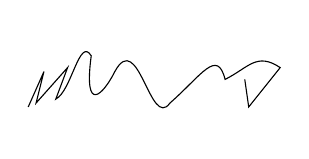
\begin{tikzpicture}
\draw(0,0)--(.2,.45)--(.1,.05)--(.5,.5)--(.35,.1)..controls(.55,.2)and(.65,.9)..(.8,.65)..controls(.7,-.1)and(.95,.15)..(1.1,.45)..controls(1.4,1)and(1.55,-.3)..(1.8,.05)..controls(2.2,.4)and(2.4,.75)..(2.5,.35)..controls(2.8,.5)and(2.9,.7)..(3.2,.5)--(2.8,0)--(2.75,.35);
\end{tikzpicture}}

\margin{19}
